\chapter{Resultados}



\section{Resultados de simulação}

\begin{figure}[H]
    \centering
    \includegraphics[width=0.8\linewidth]{figuras/simulacao_referencia_01m.eps}
    \caption[Simulação do controlador com referência de 0,1 m]{Simulação do controlador com referência de 0,1 m.}
    \label{fig:simulacao01m}
\end{figure}

\begin{figure}[H]
    \centering
    \includegraphics[width=0.8\linewidth]{figuras/simulacao_referencia_02m.eps}
    \caption[Simulação do controlador com referência de 0,2 m]{Simulação do controlador com referência de 0,2 m.}
    \label{fig:simulacao02m}
\end{figure}

\begin{figure}[H]
    \centering
    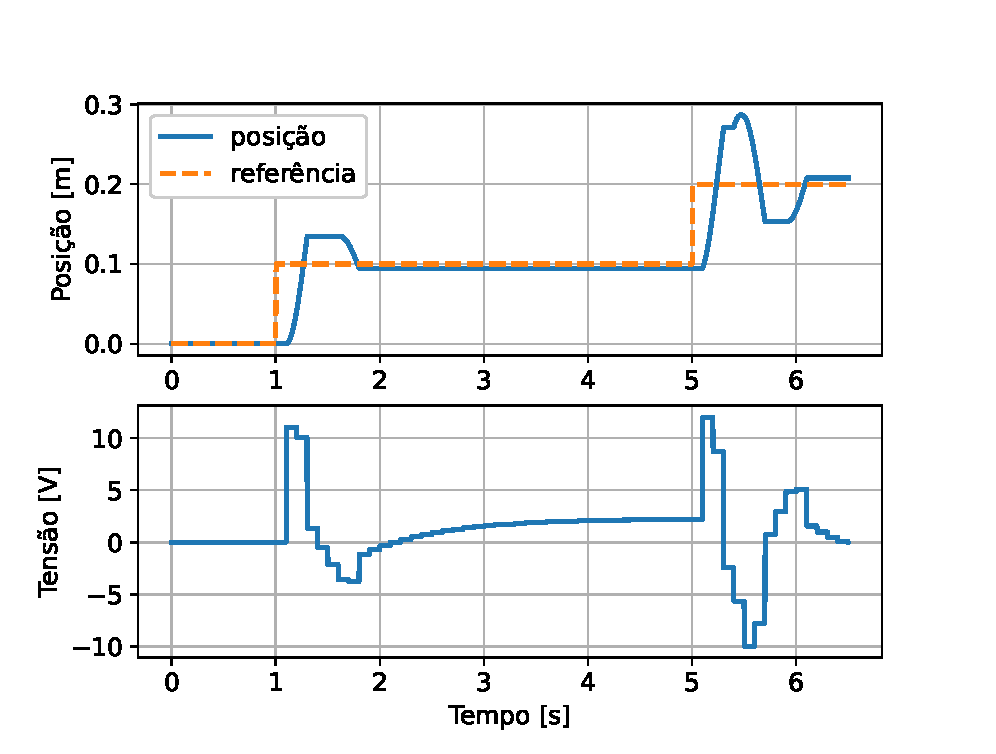
\includegraphics[width=0.8\linewidth]{figuras/simulacao_referencia_01e02m.eps}
    \caption[Simulação do controlador com referência de 0,1 m e 0,2 m]{Simulação do controlador com referência de 0,1 m e 0,2 m.}
    \label{fig:simulacao01e02m}
\end{figure}

\section{Resultados experimentais}

\begin{figure}[H]
    \centering
    \includegraphics[width=0.8\linewidth]{figuras/controlador_referencia_01m.eps}
    \caption[Dados experimentais do controlador com referência de 0,1 m]{Dados experimentais do controlador com referência de 0,1 m.}
    \label{fig:controlador01m}
\end{figure}

\begin{figure}[H]
    \centering
    \includegraphics[width=0.8\linewidth]{figuras/controlador_referencia_02m.eps}
    \caption[Dados experimentais do controlador com referência de 0,2 m]{Dados experimentais do controlador com referência de 0,2 m.}
    \label{fig:controlador02m}
\end{figure}

\begin{figure}[H]
    \centering
    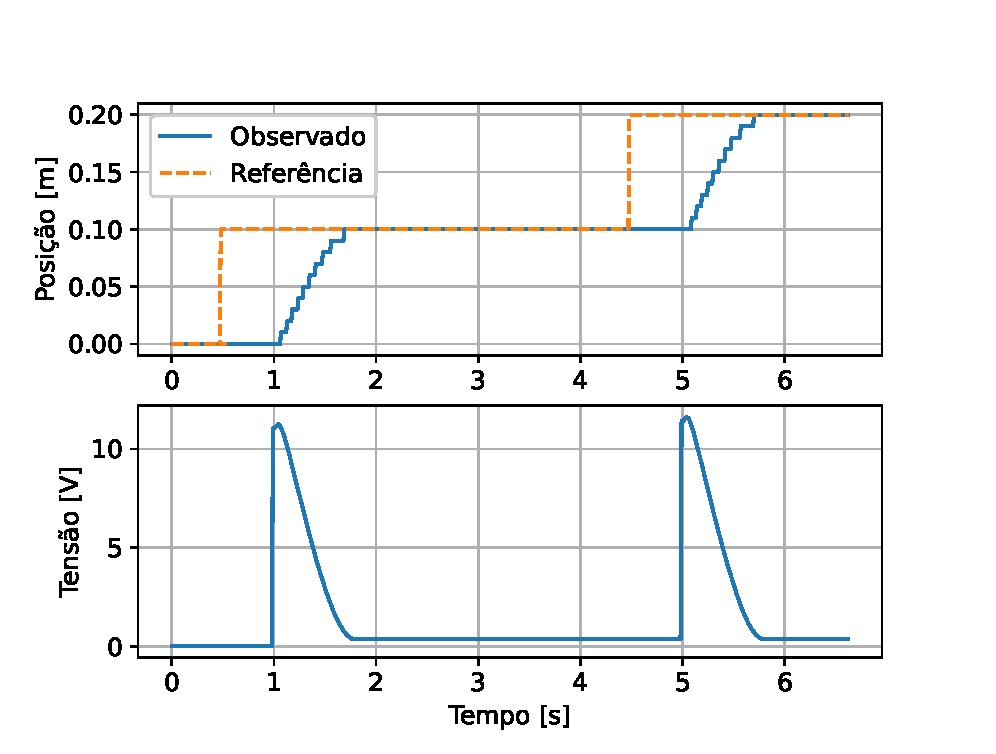
\includegraphics[width=0.8\linewidth]{figuras/controlador_referencia_01e02m.eps}
    \caption[Dados experimentais do controlador com referência de 0,1 m e 0,2 m]{Dados experimentais do controlador com referência de 0,1 m e 0,2 m.}
    \label{fig:controlador01e02m}
\end{figure}

\section{Comparação entre os Resultados}